\documentclass[e4_tp1_main.tex]{subfiles}

\begin{document}

\section{Ejercicio 1}
Se procederá al análisis del circuito de la \autoref{fig:circuit_1}. El mismo es un circuito destinado al análisis del disparo de un transistor MOSFET.


\begin{figure}[H]
  \centering
  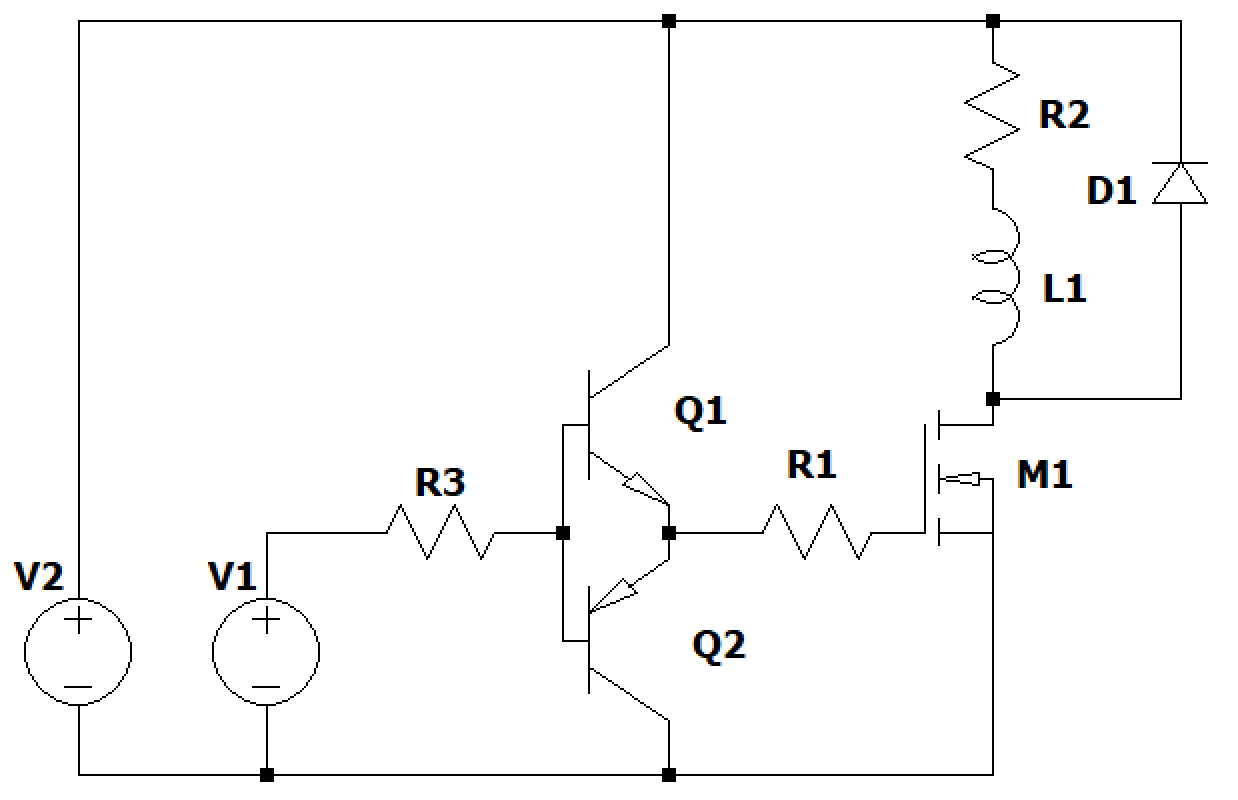
\includegraphics[width=\linewidth/2]{images/ej1/circuit_1.png}
  \caption{Circuito para análisis de disparo de transistor MOSFET}
  \label{fig:circuit_1}
\end{figure}

\subsection{Circuito Driver}

Los transistores $Q_1$ y $Q_2$ forman una configuración Totem-Pole, y se encuentran funcionando en saturación (push-pull output). 
Nótese que para prender el transistor, se requiere cargar las capacidades internas del MOSFET, por lo que se requiere un pico de corriente que un generador de señales no es capaz de proveer. Utilizando esta configuración, se puede activar y desactivar este circuito utilizando un generador de señales, mientras que la corriente es provista por la fuente de tensión.
Idealmente, la salida de este circuito valdrá $V_{out} = V_1 - 0.7V$ cuando el circuito esté activado, y $V_{out} = 0.7V$ cuando se encuentre desactivado. Este circuito afectará la curva de control del Gate, pues la misma no es un escalón ideal. Se tendrá en cuenta el delay para la interpretación de los resultados obtenidos (de ser necesario), pero no nos centraremos en el análisis de esta configuración.



\subsection{Carga Inductiva}
La carga está compuesta por un circuito RL. Para conocer las condiciones de operación de este circuito, hay que plantear las ecuaciones en funcionamiento. Estas ecuaciones son
\begin{equation}
I_1 = I_0\exp(-t_1/\tau_{RL})+\frac{V_2}{R_2}(1-\exp(-t_1/\tau_{RL}))
\end{equation}
\begin{equation}
I_0 = I_1\exp(-t_2/\tau_{RL}),
\end{equation}
donde $t_1 = D/f_s$, $t_2 = (1-D)/f_s$, $\tau_{RL}=L/R$, $f_s$ la frecuencia del switch y $D$ el duty cycle. Resolviendo el sistema de ecuaciones queda
\begin{equation}
I_0 = \frac{V_2}{R_2}\frac{1-exp(-t_1/\tau_{RL})}{exp(t_2/\tau_{RL})-exp(-t_1/\tau_{RL})}
\end{equation}
\begin{equation}
I_1 = \frac{V_2}{R_2}\frac{1-exp(-t_1/\tau_{RL})}{exp(t_2/\tau_{RL})-exp(-t_1/\tau_{RL})}\exp(t_2/\tau_{RL}).
\end{equation}
Notese que $I_0$ corresponde a la corriente en el inductor cuando se prende el MOSFET, e $I_1$ corresponde a la corriente en el inductor cuando se apaga el MOSFET.

\subsection{Conmutación MOSFET}

Durante la conmutación del MOSFET, circula corriente por el Gate. Esta corriente es debida a capacidades internas del transistor, que se cargan durante la conmutación. Dichas capacidades corresponden básicamente a las cargas de la capa de inversión e ionización que se forman en el Body del transistor para formar el canal N (Capacidad Gate-Source $C_{GS}$ - recordar que el Body y el Source se encuentran cortocircuitados internamente), y las cargas asociadas a la capa de acumulación o de depleción que se forma en el Drain del transistor (Capacidad Gate-Drain $C_{GD}$), que ayudan a minimizar la resistencia del MOSFET cuando se encuentra activado. Es importante destacar que esta capacidad depende del tamaño de la capa de acumulación / depleción, y por lo tanto cambia durante la conmutación del MOSFET. Se buscará introducir las ecuaciones a utilizar, sin entrar en detalle sobre el funcionamiento del transistor.

\subsubsection{Encendido del MOSFET}

Considerando que, ante un escalón de tensión en provisto por el circuito Driver, dichas capacidades comienzan a cargarse, se puede modelar la primera etapa del prendido del MOSFET con un circuito RC, por lo que la tensión $V_{G}$ en función del tiempo puede ser aproximada por
\begin{equation}
V_G(t) = V_1 (1-\exp(-t/\tau_1)).
\end{equation}
donde $\tau_1 = R_1\tilde{C}_{G,1}$ y $\tilde{C}_{G,1} = C_{GS} + C_{GD,1}$. Cuando la tensión en el Gate llega a $V_{GS,th}$ (en $t=t_{d,on}$), comienza a formarse la capa de inversión, por lo que la corriente del Drain $I_D$ comienza a aumentar hasta llegar al valor $I_0$ impuesto por la carga inductiva y hasta que el diodo deje de conducir (en $t=t_1$). Esto ocurrirá cuando la tensión en el Gate llegue a un valor $V_G=V_{G,I_D=I_0}$. El tiempo entre que comienza a circular corriente hasta que se alcanza el valor $I_0$ se denomina $t_{ri}$. Se puede demostrar que

\begin{equation}
t_{d,on} = -\tau_1 \ln\left(1-\frac{V_{G,th}}{V_1}\right)
\end{equation}
\begin{equation}
t_{1} = -\tau_1 \ln\left(1-\frac{V_{G,I_D=I_0}}{V_1}\right)
\end{equation}
\begin{equation}
t_{ri} = t_{1} - t_{d,on}.
\end{equation}

Luego, cuando la corriente de Drain llega al valor $I_0$, el valor de la tensión en el Gate se mantiene temporalmente en $V_G=V_{G,I_D=I_0}$, por lo que la capacidad $C_{GS}$ deja de cargarse, mientras se sigue cargando $C_{GD}$ a corriente constante. A medida se cargue $C_{GD}$ se formará la capa de acumulación, bajando la resistencia $R_{DS}$, por lo que disminuye la tensión $V_{DS}$ hasta alcanzar el valor $V_{DS,on}$. Dado que la capacidad $C_{GD}$ varía durante este proceso, pues varían la longitud de la capa de acumulación, suele utilizarse el valor de la carga total $\Delta Q$ para estimar la duración de esta etapa. Con esto, el tiempo que transcurre desde que empieza a caer la tensión $V_{DS}$ hasta que alcanza el valor $V_{DS,on}$ puede estimarse según:

\begin{equation}
t_{fv} = \Delta Q/I_{G,on} = \frac{\Delta Q R_1}{V_{1}-V_{G,I_D=I_0}}
\end{equation}

A lo largo de esta etapa, cambia el valor de $C_{GD}$ de $C_{GD,1}$ a $C_{GD,2}$. El cambio de la tensión $V_{DG}$ en función del tiempo puede expresarse según

\begin{equation}
\frac{dV_{DG}}{dt} = \frac{V_{GG}-V_{G,I_D=I_0}}{R_1C_{GD}}.
\end{equation}

Una aproximación es considerar que esto ocurre en dos etapas: una donde $C_{GD} = C_{GD,1}$ y otra donde $C_{GD} = C_{GD,2}$. 

Luego, la tensión en el Gate sigue creciendo hasta llegar al valor $V_{GG}$. El tiempo característico asociado está dado por:

\begin{equation}
\tau_2 = R_1\tilde{C}_{G,2}
\end{equation}
Donde $\tilde{C}_{G,2} = C_{GS} + C_{GD,2}$

\subsubsection{Apagado del MOSFET}

El apagado del MOSFET es similar al encendido, pero en orden contrario:

Primero, se comienzan a descargar las capacidades internas por el Gate, por lo que la tensión del Gate en la primera etapa está dada por:

\begin{equation}
V_G(t) = V_{GG} \exp(-t/\tau_2)
\end{equation}

Esto ocurrirá hasta que la tensión $V_G$ alcance el valor $V_{G,I_D=I_0}$ en $t=t_{d,off}$. Puede demostrarse que:
\begin{equation}
t_{d,off}= -\tau_2\ln\left(\frac{V_{G,I_D=I_0}}{V_{GG}}\right)
\end{equation}

Luego, la tensión en el Gate permanecerá constante mientras se descarga $C_{GD,2}$ a corriente constante durante un tiempo $t_{rv}$. Análogo al caso de encendido, este tiempo está dado por
\begin{equation}
t_{rv} = \Delta Q/I_{G,off} = \frac{\Delta Q R_1}{V_{G,I_D=I_0}}
\end{equation}

Notar que, al igual que durante el prendido, la capacidad $C_{GD}$ cambia de valor durante este proceso. La misma aproximación en dos etapas aplica para este caso. Finalmente, la tensión en el Gate baja según la ecuación
\begin{equation}
V_{G} = V_{G,I_D=I_0}\exp(-t/\tau_1).
\end{equation}

A medida que la tensión cae, comienza a deshacerse el canal formado, por lo que baja el valor de $I_D$ hasta hacerse nulo cuando $V_G=V_{G,th}$. Esto ocurre luego de un intervalo $t_{fi}$. El valor de $t_{fi}$ está dado por
\begin{equation}
t_{fi}= -\tau_1\ln\left(\frac{V_{G,th}}{V_{G,I_D=I_0}}\right).
\end{equation}

Un gráfico esquemático mostrando la conmutación del MOSFET se muestra en la \autoref{fig:mosfet_theory}.


\begin{figure}[H]
  \centering
  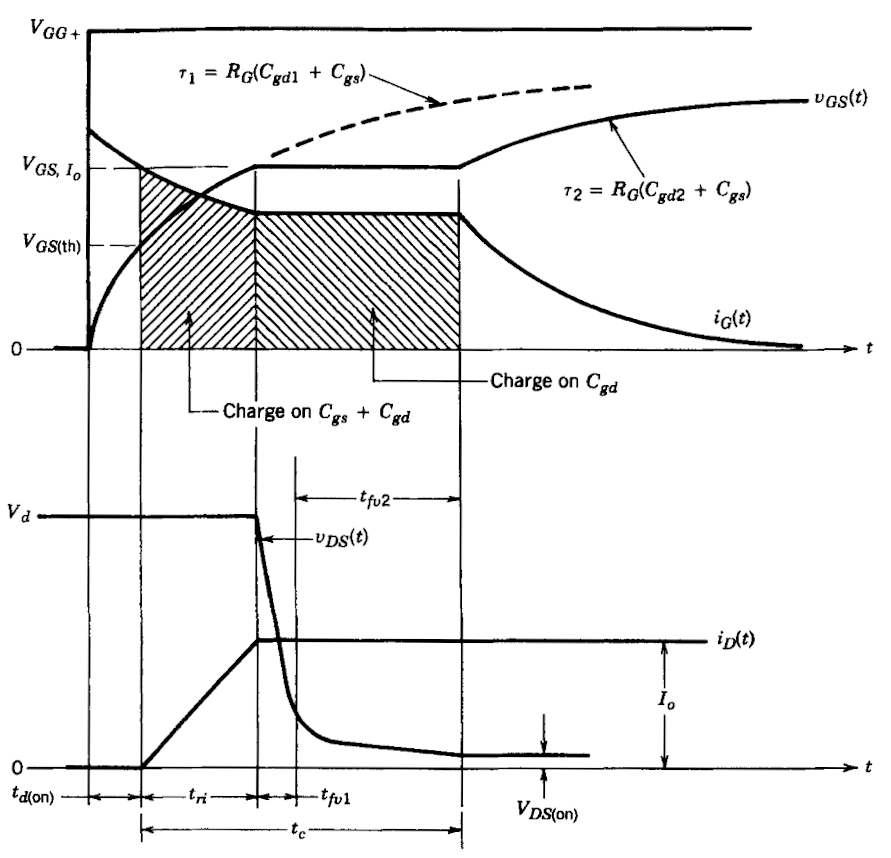
\includegraphics[width=\linewidth/2]{images/ej1/theory_mosfet.png}
  \caption{Curvas de tensión y corriente en el MOSFET durante el encendido}
  \label{fig:mosfet_theory}
\end{figure}

\subsection{Diodo}
También resulta importante analizar la dinámica del Diodo durante la conmutación, dado que afecta a las curvas de conmutación del MOSFET, que es lo que se busca analizar en este punto. Con este objetivo, se realizará un breve análisis de la conmutación de un diodo real. El análisis se realiza considerando un switch que impone un cambio de corriente $di/dt$. Recordar que un diodo de potencia está formado por dos junturas: $p^+n^-n^+$.

\begin{figure}[H]
  \centering
  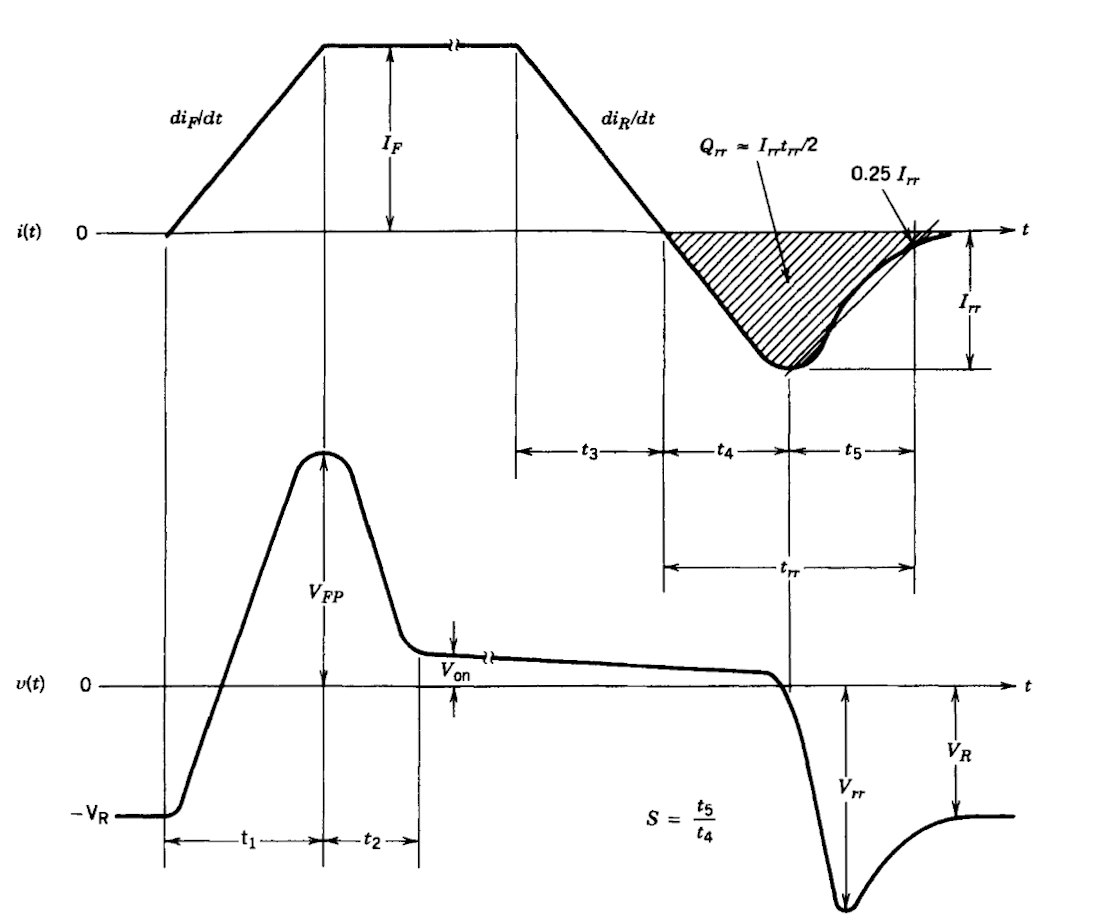
\includegraphics[width=\linewidth/2]{images/ej1/diode.png}
  \caption{Curvas de encendido y de apagado de un diodo de potencia (tensión y corriente)}
  \label{fig:diode}
\end{figure}

\subsubsection{Encendido del Diodo} 
Cuando el diodo se encuentra polarizado en inversa y se lo prende, la corriente sube de acuerdo con el $di/dt$ impuesto por el circuito, a medida que se restaura la carga en la zona de depleción hasta el valor de equilibrio térmico y se comienza a polarizar en directa. A medida que el diodo se polariza en directa, baja su la resistencia hasta que la tensión en el diodo llega a $V_{on}$. Por la corriente que circula mientras que el diodo no está completamente polarizado, motivo por el cual su resistencia interna es alta, se produce un pico de tensión en el diodo. Este pico puede resultar mayor considerando las inductancias parásitas, si se aplican valores altos de $di/dt$. Este overshoot puede afectar seriamente algunos circuitos de potencia. La curva de encendido del diodo se puede encontrar en la \autoref{fig:diode}.

\subsubsection{Apagado del Diodo}
El apagado del diodo es esencialmente el proceso inverso al encendido. Primero, los portadores de carga libres deben ser removidos para que la juntura llegue al equilibrio térmico antes de que la misma pueda ser polarizada en inversa. Siempre que haya exceso de portadores de carga libre en las zonas de drift, las junturas estarán polarizadas en directa, por lo que la tensión en el diodo no varia más alla de pequeñas diferencias por pérdidas ohmicas. Una vez que suficientes portadores de carga sean removidos y la corriente se vuelva negativa, la o las junturas se polarizan en inversa, momento en el que la corriente deja de volverse más negativa y tiende al valor de cero. Este pico de corriente negativo se denomina $I_{rr}$. Durante este último intervalo hay pérdidas de potencia debido a que crece la resistencia del diodo al polarizarse en inversa, por lo que hay un pico de tensión negativo, y luego la corriente tiende a cero (y la tensión baja en módulo y tiende al valor de tensión aplicado en el diodo). La curva de apagado del diodo se puede encontrar en la \autoref{fig:diode}.

\subsubsection{Efecto de $I_{rr}$ en la conmutación del MOSFET}
\label{subsubsec:irr_effect}

El valor de $I_{rr}$ afecta en la conmutación del MOSFET. Nótese que este efecto se da cuando el diodo se apaga, es decir, durante el encendido del MOSFET.

Por causa de la corriente $I_{rr}$, la corriente de Drain $I_D$ crece hasta el valor $I_0+I_{rr}$, por lo que el valor de $V_{G}$ crece por arriba de $V_{G,I_D=I_0}$. Cuando el diodo se recupera y la corriente vuelve a cero (y, por lo tanto, la corriente $I_D$ baja a $I_0$), el valor de $V_G$ baja a $V_{G,I_D=I_0}$, y el cambio de tensión provee corriente adicional a la capacidad $C_{GD}$, produciendo que $V_{GD}$ y $V_{DS}$ decrezcan rápidamente durante este intervalo de recovery. Los efectos de la corriente $I_{rr}$ en la conmutación del MOSFET pueden observarse en la \autoref{fig:mosfet_irr}.

\begin{figure}[H]
  \centering
  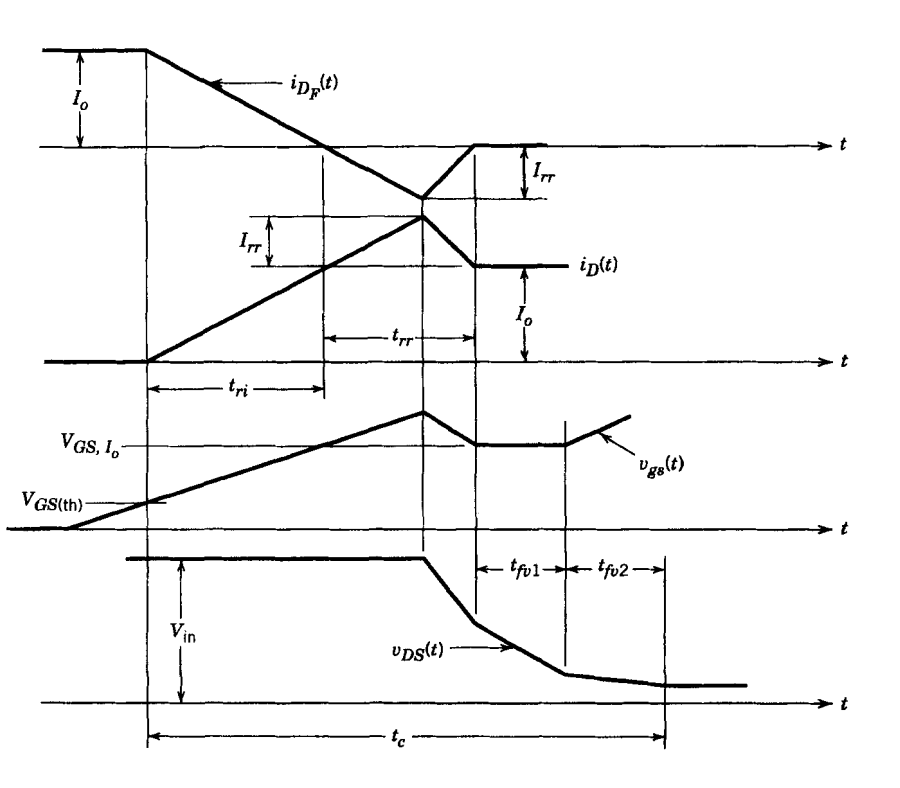
\includegraphics[width=\linewidth/2]{images/ej1/diode_irr.png}
  \caption{Efectos de $I_{rr}$ en el encendido del MOSFET.}
  \label{fig:mosfet_irr}
\end{figure}

Esta corriente no se tendrá en cuenta para el análisis teórico.

\subsection{Valores de los componentes y variables}

Los valores de los componentes y las variables se muestran en la \autoref{tab:values_1} y la \autoref{tab:values_2}.

\begin{table}[H]
\centering
\begin{tabular}{|c|c|c|c|c|c|}
\hline
Componente & $Q_1$ & $Q_2$ & $R_1$ & $R_2$ & $R_3$ \\
\hline
Valor & BC337-25 & BC557B & 100 $\Omega$ & 15 $\Omega$ & 1 $K\Omega$ \\
\hline
Componente & $M_1$ & $L_1$ & $D_1$ & $V_2$ & $V_1$\\
\hline
Valor & IRF530 & 220 $\mu H$ & MUR460 & 50 V & Ver Tabla $V_1$\\
\hline
\end{tabular}
\caption{Valores de los componentes utilizados.}
\label{tab:values_1}
\end{table}

\begin{table}[H]
\centering
\begin{tabular}{|c|c|}
\hline
Parámetro & Valor \\
\hline
$V_0$ (on) & $15$ V \\
\hline
$V_0$ (off) & $0$ V \\
\hline
$f_s$ & $50$ KHz \\
\hline
$D$ (Duty Cycle) & $50\%$ \\
\hline
\end{tabular}
\caption{Valores asociados a generador de $V_1$.}
\label{tab:values_2}
\end{table}

\subsection{Búsqueda de parámetros en datasheet y cálculo de valores}

Los valores de los parámetros del circuito obtenidos a partir del datasheet del transistor se muestran en la \autoref{tab:obtained_values_1} y la \autoref{tab:obtained_values_2}.\\
\begin{table}[H]
\centering
\begin{tabular}{|c|c|c|c|c|c|c|c|c|c|}
\hline
Variable & $I_{0_{off}}$ & $I_{0_{on}}$ & $V_{G,th}$ & $V_{G,I_D=I_{0_{off}}}$   & $V_{G,I_D=I_{0_{on}}}$ & $\tilde{C}_{G,1}$ & $\tilde{C}_{GD,2}$ & $\Delta Q$  \\
\hline
Valor & 2,21 A & 1,12 A & 4 V & 4,8 V & 4,5 V & 650 pF & 1120 pF & 7 nC\\
\hline
\end{tabular}
\caption{Valores obtenidos del datasheet}
\label{tab:obtained_values_1}
\end{table}

\begin{table}[H]
\centering
\begin{tabular}{|c|c|c|c|}
\hline
Variable & $C_{gd,1}$ & $C_{gd,2}$ & $C_{gs}$\\
\hline
Valor & 50 pF & 520 pF & 600 pF\\
\hline
\end{tabular}
\caption{Valores de los capacitores}
\label{tab:obtained_values_2}
\end{table}

Los tiempos de conmutación teóricos se muestran en la \autoref{tab:conmutation_times_theory}.

\begin{table}[H]
\centering
\begin{tabular}{|c|c|c|c|c|c|c|c|c|}
\hline
Variable & $t_{d,on}$ & $t_{ri}$ & $t_{fv}$ & $t_{d,off}$ & $t_{rv}$ & $t_{fi}$  \\
\hline
Valor & $21.32$ ns & $3.23$ ns & $71.43$ ns & $127.62$ ns & $145.83$ ns & $11.85$ ns\\
\hline
\end{tabular}	
\caption{Tiempos de conmutación calculados}
\label{tab:conmutation_times_theory}
\end{table}

\subsection{Curvas teóricas}
Las curvas obtenidas a partir de la teoría se muestran en la \autoref{fig:teoria}.

\begin{figure}
  \centering
  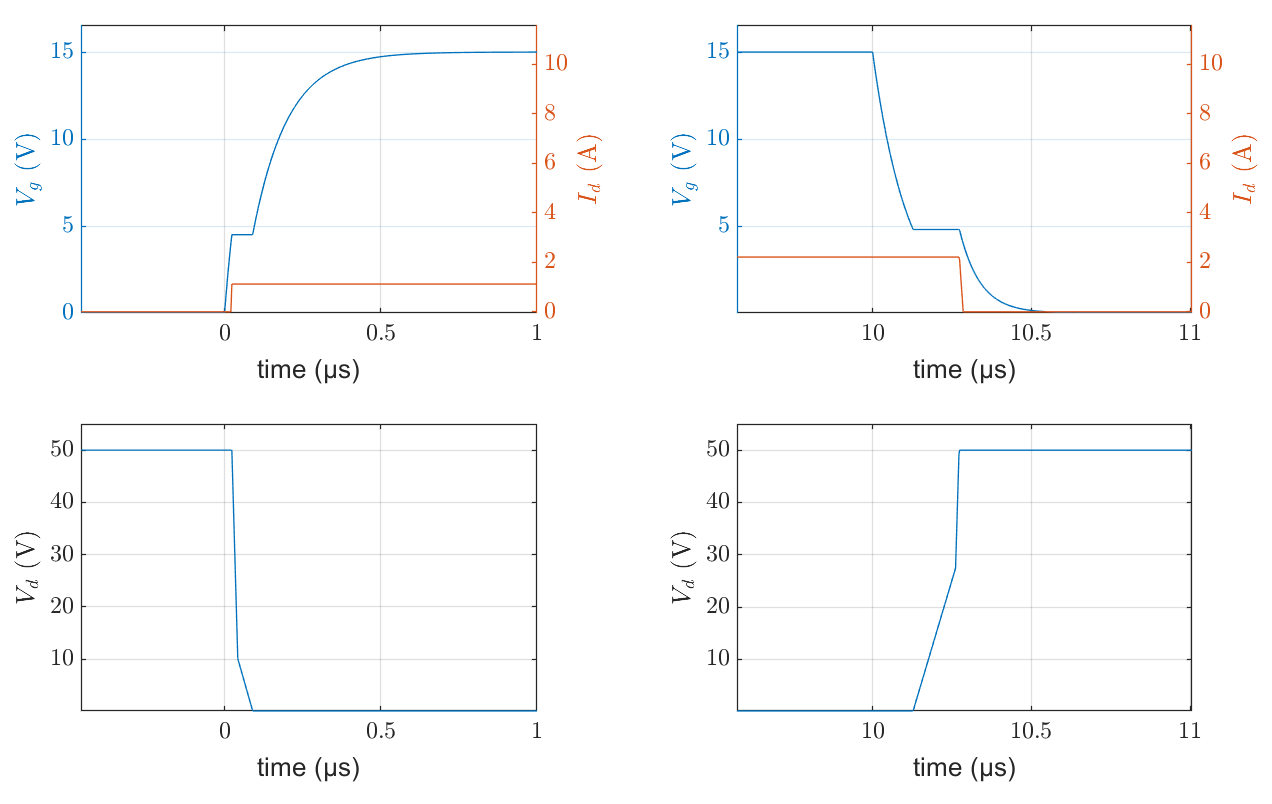
\includegraphics[width=\linewidth]{images/ej1/curvas_teoria.png}
  \caption{Curvas teóricas de $V_G$, $V_{DS}$ e $I_D$.}
  \label{fig:teoria}
\end{figure}


\subsection{Curvas Simuladas y valores obtenidos con la simulación}
Las curvas de conmutación obtenidas en la simulación pueden observarse en la \autoref{fig:simulation}. Los valores de los tiempos de conmutación obtenidos a partir de la simulación se muestran en la \autoref{tab:conmutation_times_simulation}
\begin{table}[H]
\centering
\begin{tabular}{|c|c|c|c|c|c|c|c|c|}
\hline
Variable & $t_{d,on}$ & $t_{ri}$ & $t_{fv}$ & $t_{d,off}$ & $t_{rv}$ & $t_{fi}$  \\
\hline
Valor & $28$ ns & $12$ ns & $183$ ns & $170$ ns & $450$ ns & $13$ ns\\
\hline
\end{tabular}	
\caption{Tiempos de conmutación obtenidos a partir de la simulación.}
\label{tab:conmutation_times_simulation}
\end{table}

\begin{landscape}
\begin{figure}
  \centering
  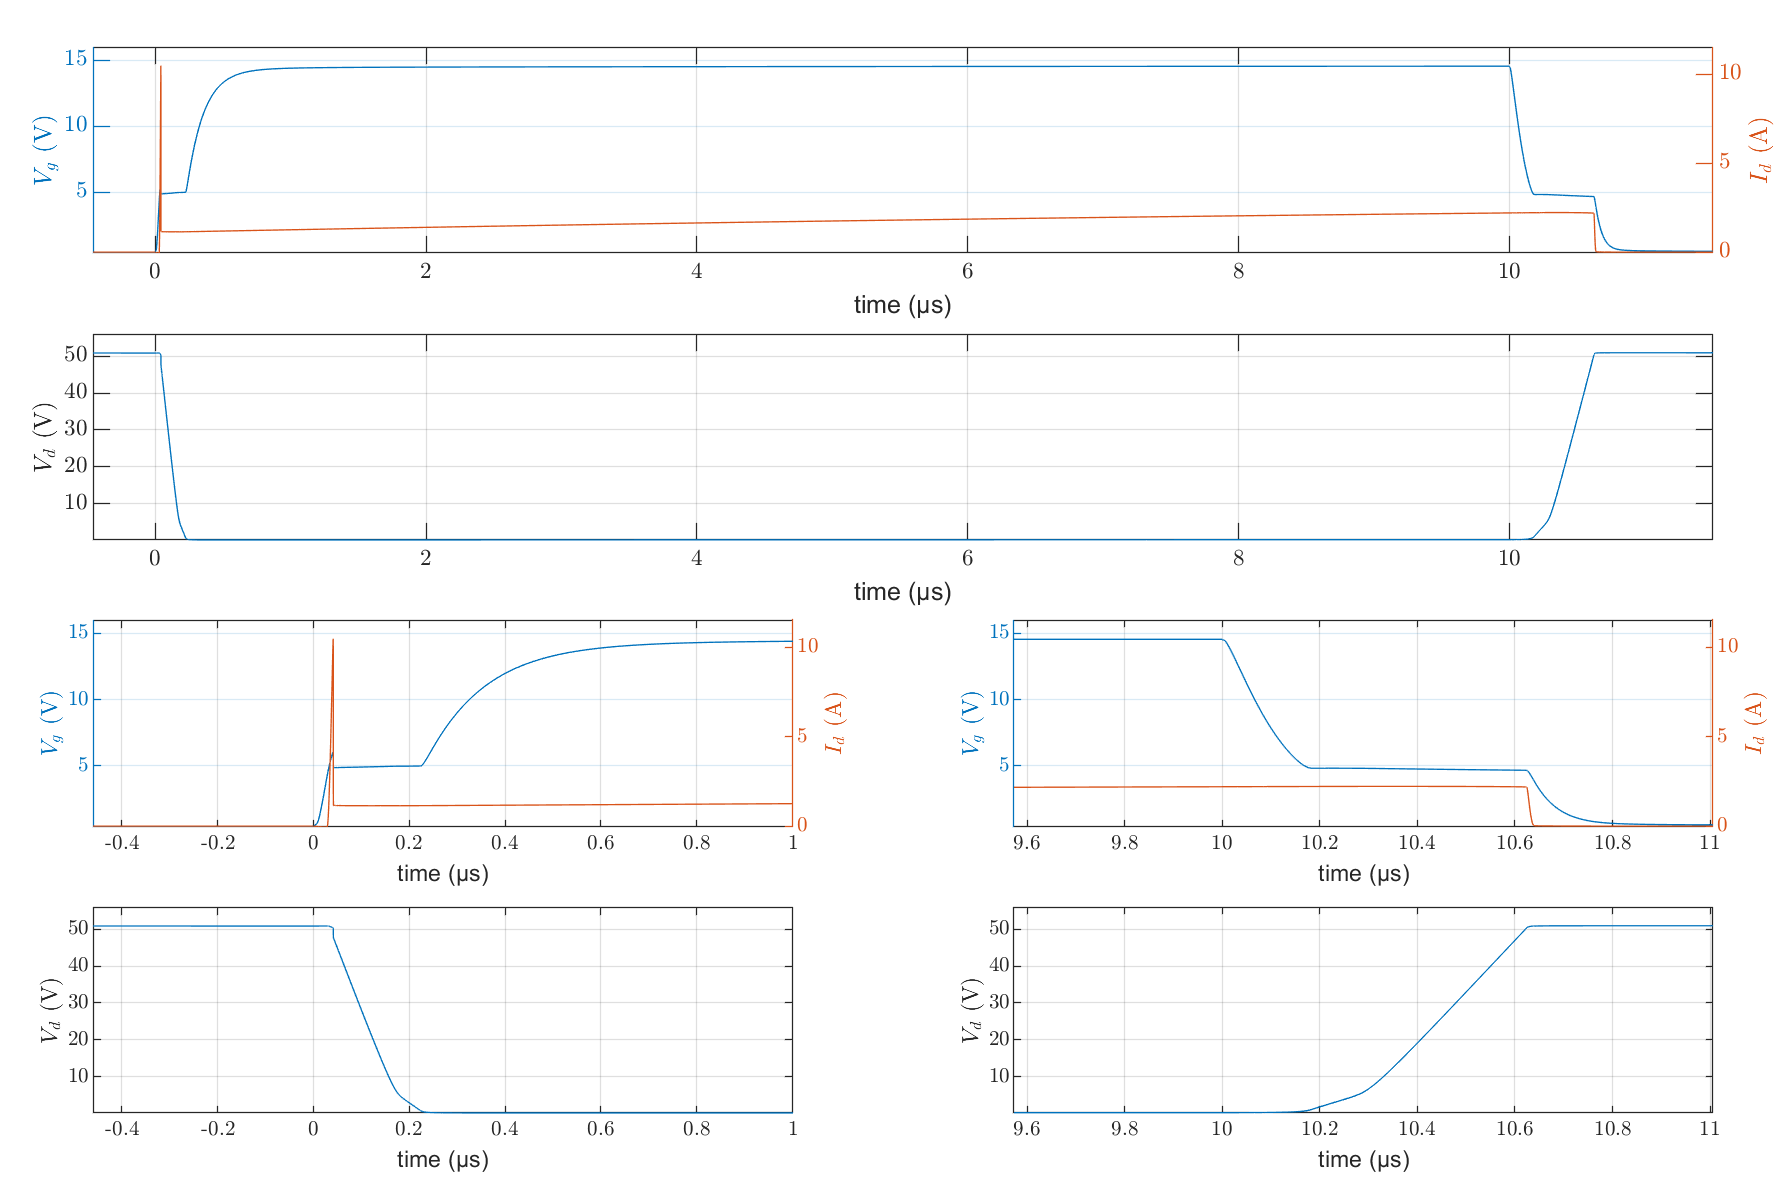
\includegraphics[width=\linewidth]{images/ej1/curvas_simuladas.png}
  \caption{Curvas simuladas de $V_G$, $V_{DS}$ e $I_D$, y detalle de conmutación de encendido y apagado.}
  \label{fig:simulation}
\end{figure}
\end{landscape}

\subsection{Comparación de resultados obtenidos}
Al comparar los resultados teóricos y las simulaciones, la diferencia más significativa es el pico de corriente que aparece en la corriente de Drain $I_D$. Este pico es debido a la corriente $I_{rr}$ desarrollada en la \autoref{subsubsec:irr_effect}. Este efecto no fue considerado para graficar las curvas teóricas, pero los resultados obtenidos en la simulación ($I_{D,max}=10.29A$, cuando $I_0 = 1.15A$) muestran la importancia de tener en consideración este análisis.

Con respecto a la forma de las curvas obtenidas, las curvas teóricas y simuladas resultan semejantes en forma, con desviaciones por la aproximación del modelo teórico con respecto al modelo de la simulación, presentando algunas diferencias en los tiempos de las distintas etapas de la conmutación. 


Los tiempos de las distintas etapas obtenidos con la simulación difieren de los valores calculados teóricamente. Este resultado es de esperar, dado que los valores utilizados y obtenidos a partir del datasheet pueden diferir con respecto a los valores tanto del componente real como de aquellos utilizados en el modelo de la simulación. Sin embargo, los valores son comparables en cuanto a su orden de magnitud. Se muestra en la \autoref{tab:error_times} los errores relativos porcentuales de los tiempos de conmutación, asi como la diferencia de orden de magnitud entre los valores teóricos y simulados.

\begin{table}[H]
\centering
\begin{tabular}{|c|c|c|c|c|c|c|}
\hline
Variable & $t_{d,on}$ & $t_{ri}$ & $t_{fv}$ & $t_{d,off}$ & $t_{rv}$ & $t_{fi}$  \\
\hline
Error porcentual & $23.8\% $ & $73\%$  & $60.9\%$  & $24.9\%$  & $67.5\%$  & $8.84\%$ \\
\hline
$\log_{10}$(Teórico/Simulado) & $-0.11$ & $-0.56$  & $-0.4$  & $-0.12$  & $-0.48$  & $-0.04$ \\
\hline
\end{tabular}	
\caption{Errores porcentuales y diferencias en orden de magnitud de tiempos de conmutación.}
\label{tab:error_times}
\end{table}

Se puede observar que las diferencias más importantes se dan para los valores de $t_{d,on}$, $t_{fv}$ y $t_{rv}$. Es de esperar una desviación en el valor de $t_{d,on}$ con respecto al calculado teóricamente, por los efectos de la corriente $I_{rr}$. Con respecto a las desviaciones de los valores de $t_{fv}$ y $t_{rv}$, estos dos valores presentan desviaciones similares, y ambos están asociados al valor de la carga $\Delta Q$, por lo que un posible motivo de estas desviaciones es que el valor de $\Delta Q$ obtenido a partir del datasheet para calcular los valores de $t_{fv}$ y $t_{rv}$ difieren del valor utilizado para el modelo de la simulación.
\begin{figure}[H]
  \centering
  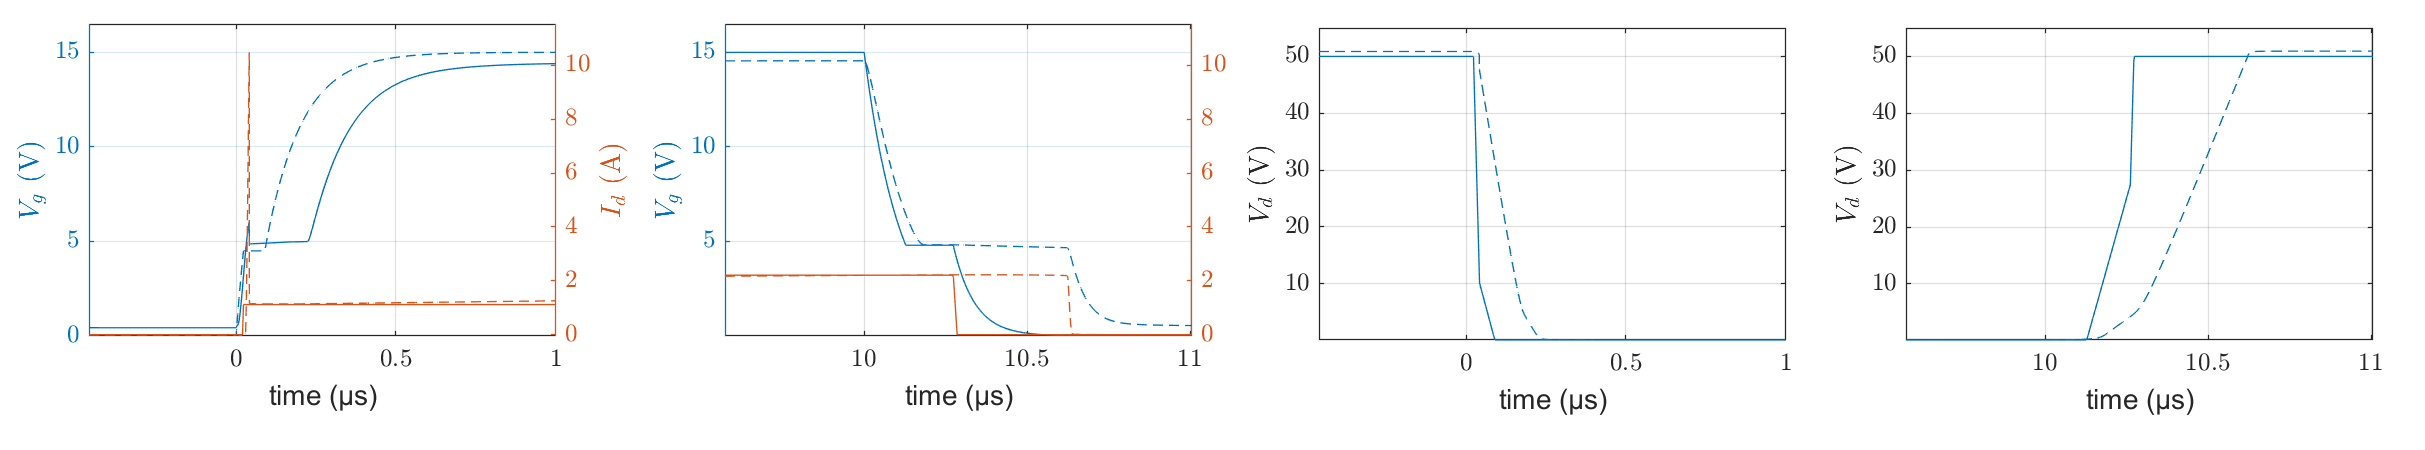
\includegraphics[width=\linewidth]{images/ej1/comparison.png}
  \caption{Superposición de curvas simuladas (lineas sólidas) y obtenidas a partir de la teoría (lineas discontinuas). }
  \label{fig:comparison}
\end{figure}


\end{document}
